\documentclass[../main.tex]{subfiles}

\begin{document}

    \subsection{Modele procesu testowego}

    \subsubsection{TMAP lifecycle model}

    \begin{figure}[H]
        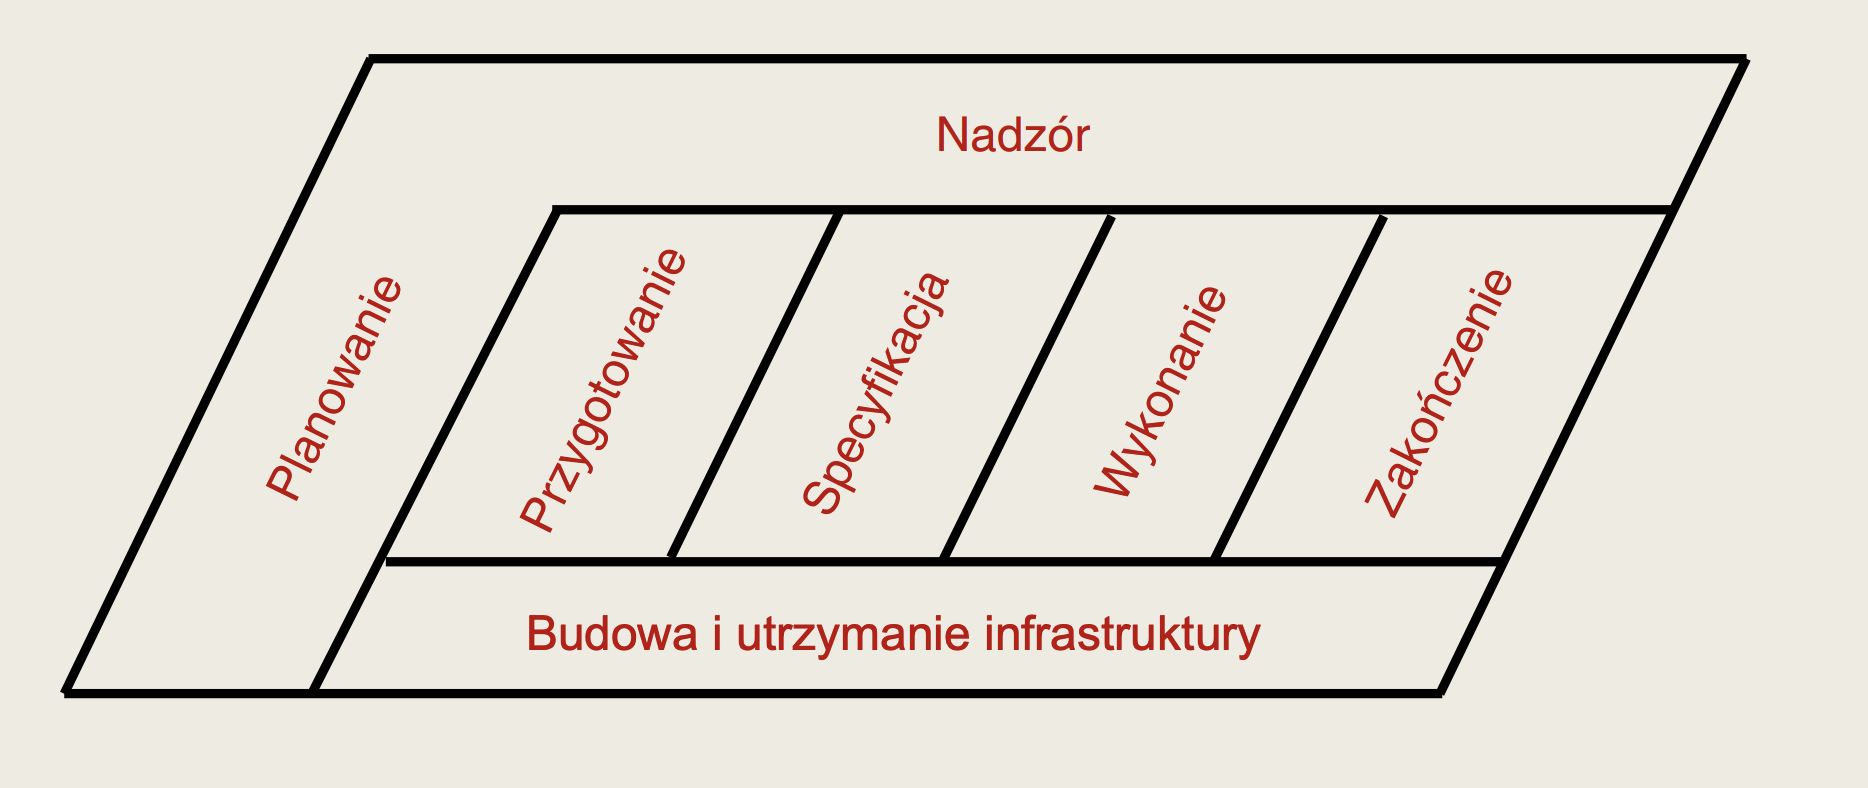
\includegraphics[width=\linewidth]{tmap.png}
    \end{figure}

    Proces jest \textbf{generyczny}, tzn. może być stosowany do wszystkich
    poziomów i typów testów. Każda faza dzieli się na określone czynności.


    \subsubsection{ISO 29119}

    \begin{figure}[H]
        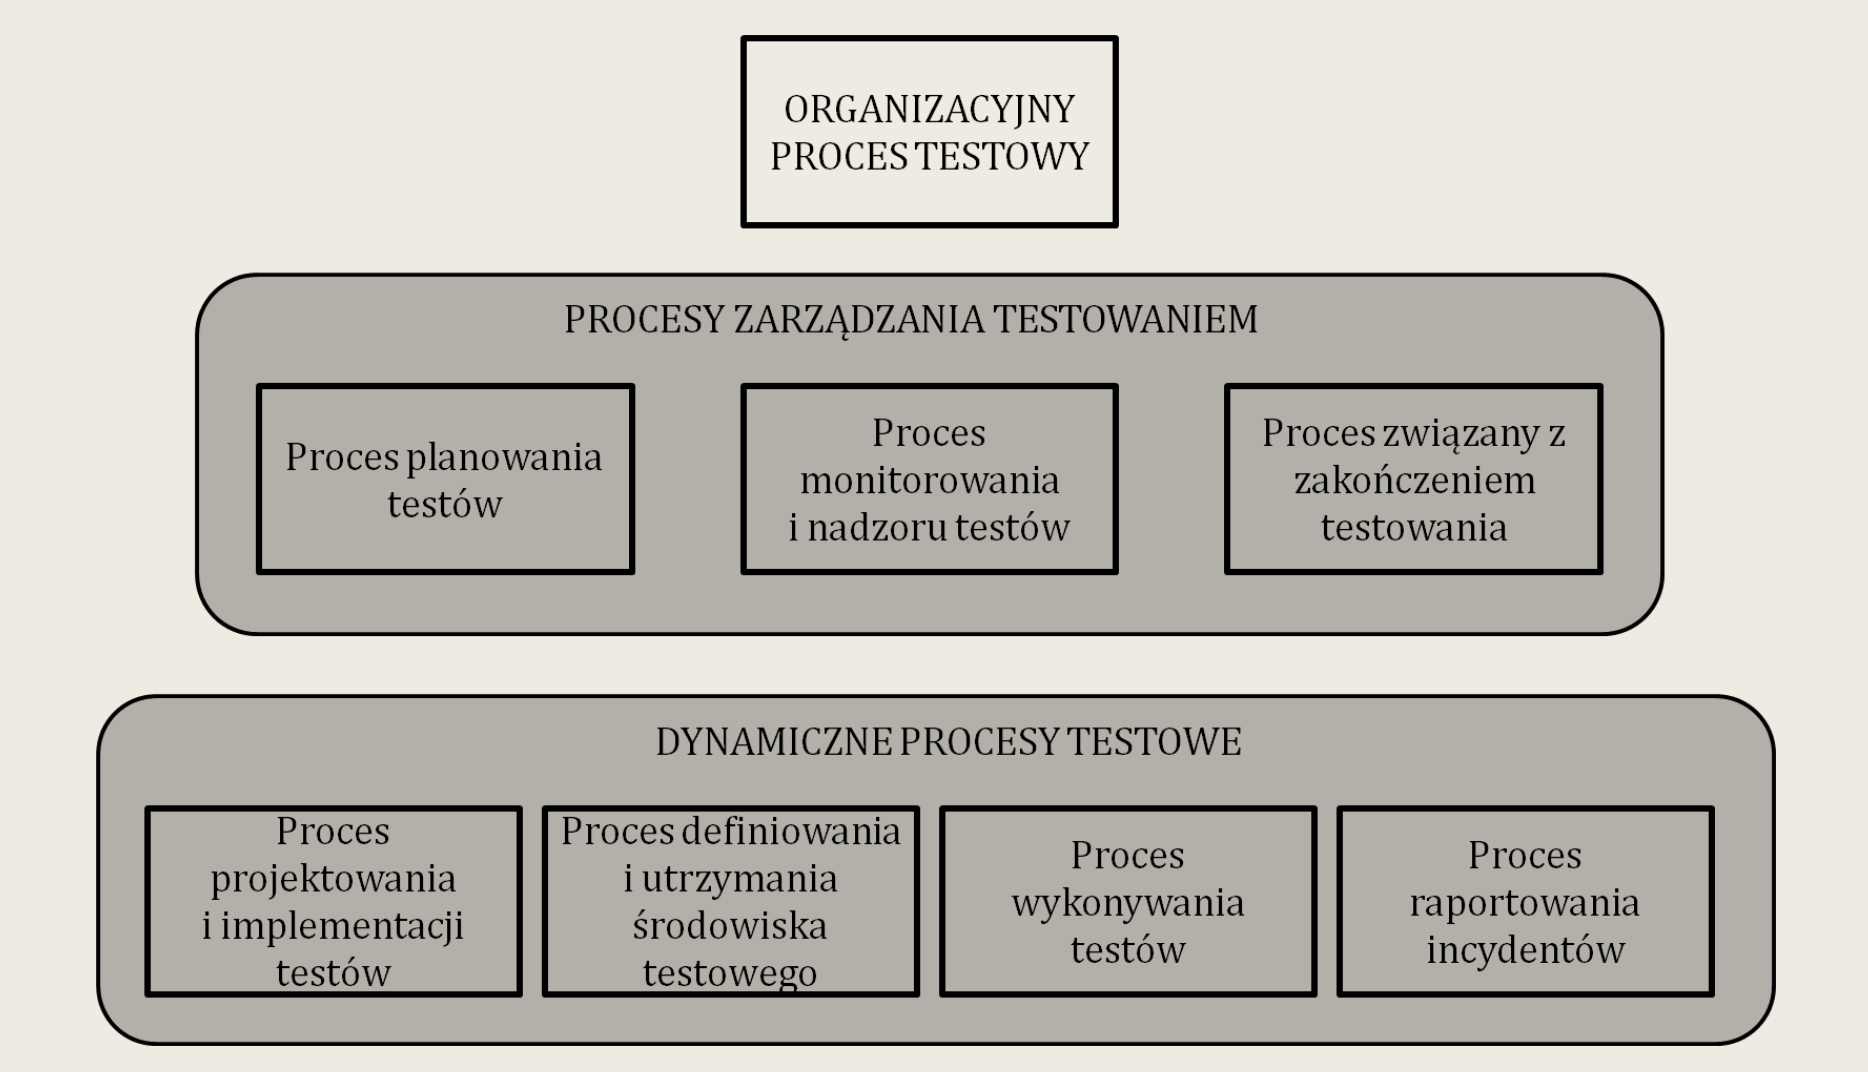
\includegraphics[width=\linewidth]{iso29119.png}
    \end{figure}


    \subsection{Miejsce testowania w modelu cyklu życia.}

    \textbf{Testowanie musi wpasować się w jakiś model.}

    \textbf{Cechy dobrego testowania.}
    \begin{itemize}
        \item każdej czynności wytwórczej odpowiada czynność związana z testowaniem
        \item każdy poziom testowania ma zdefiniowane cele
        \item analiza i projektowanie testów dla danego poziomu powinny rozpoczynać się już podczas odpowiadającej
        im fazy wytwarzania
        \item testerzy powinni uczestniczyć w przeglądach już od wczesnych wersji dokumentacji tworzonej podczas wytwarzania
    \end{itemize}

    \textbf{Poziomy a typy testów.}\\
    Poziomy testów są \textbf{ortogonalne} do typów testów, tzn.:
    \begin{itemize}
        \item na danym poziomie testów można wykonywać dowolne typy testów
        \item dany typ testów może być wykorzystany na dowolnym poziomie
    \end{itemize}

    Oczywiście niektóre typy i poziomy są silniej ze sobą powiązane, np.:
    \begin{itemize}
        \item testy jednostkowe to zazwyczaj testy oparte na strukturze
        \item na etapie testów akceptacyjnych raczej stosuje się testy
        funkcjonalne i niefunkcjonalne
        \item testy funkcjonalne zazwyczaj oparte są na specyfikacji (black-box)
        \item testy integracyjne zazwyczaj dotyczą funkcjonalności
    \end{itemize}


    \subsection{Poziomy testów.}

    \textbf{Poziom testów} określa \textbf{sposób} testowania ze względu na \textbf{postać}
    testowanego obiektu w kontekście cyklu życia (\textbf{co testujemy?}).

    \subsubsection{Testy jednostkowe.}
    \begin{tabular}{|p{3cm}|p{13cm}|}
        \hline
        \textbf{Podstawa testów} & wymagania na moduły, projekt szczegółowy, kod\\
        \hline
        \textbf{Typowe obiekty} & testów moduły, programy, funkcje, klasy, procedury\\
        \hline
    \end{tabular}

    \begin{itemize}
        \item inne nazwy: testowanie modułowe, unit testing
        \item defekty szukane w izolacji od reszty systemu
        \item wykorzystanie zaślepek i sterowników
        \item wykorzystanie frameworków do testów jednostkowych i debugowania
        \item przeprowadzane przez deweloperów – autorów testowanego kodu
        \item usuwanie defektów bezpośrednio po znalezieniu
        \item brak formalnego procesu zarządzania defektami
    \end{itemize}

    \textbf{TTD} - Test Driven Developement.
    \begin{itemize}
        \item \textbf{Napisanie testu} - sprawdza, że programista rozumie zachowanie nowego kodu
        \item \textbf{Uruchomienie testu}, który jest nie zdany(testuje uprząż testową i sam test; pokazuje,
        że wystąpi awaria, gdy kod będzie błędny)
        \item \textbf{Napisanie kodu} w minimalnej ilości, wystarczającej do zdania testu; jeśli
        konieczne, dokonanie refaktoryzacji
    \end{itemize}

    \subsubsection{Testy integracyjne.}
    \begin{tabular}{|p{3cm}|p{13cm}|}
        \hline
        \textbf{Podstawa testów} & projekt systemu, architektura, przypadki użycia\\
        \hline
        \textbf{Typowe obiekty} & interfejsy, podsystemy, konfiguracje systemów\\
        \hline
    \end{tabular}

    \begin{itemize}
        \item testuje interfejsy i interakcje
        \item im większy zakres integracji, tym trudniej izolować defekty
        \item rozumienie architektury testowanych modułów/systemów
        \item może odbywać się na wielu poziomach (np. integracja systemów)
    \end{itemize}

    \begin{figure}[H]
        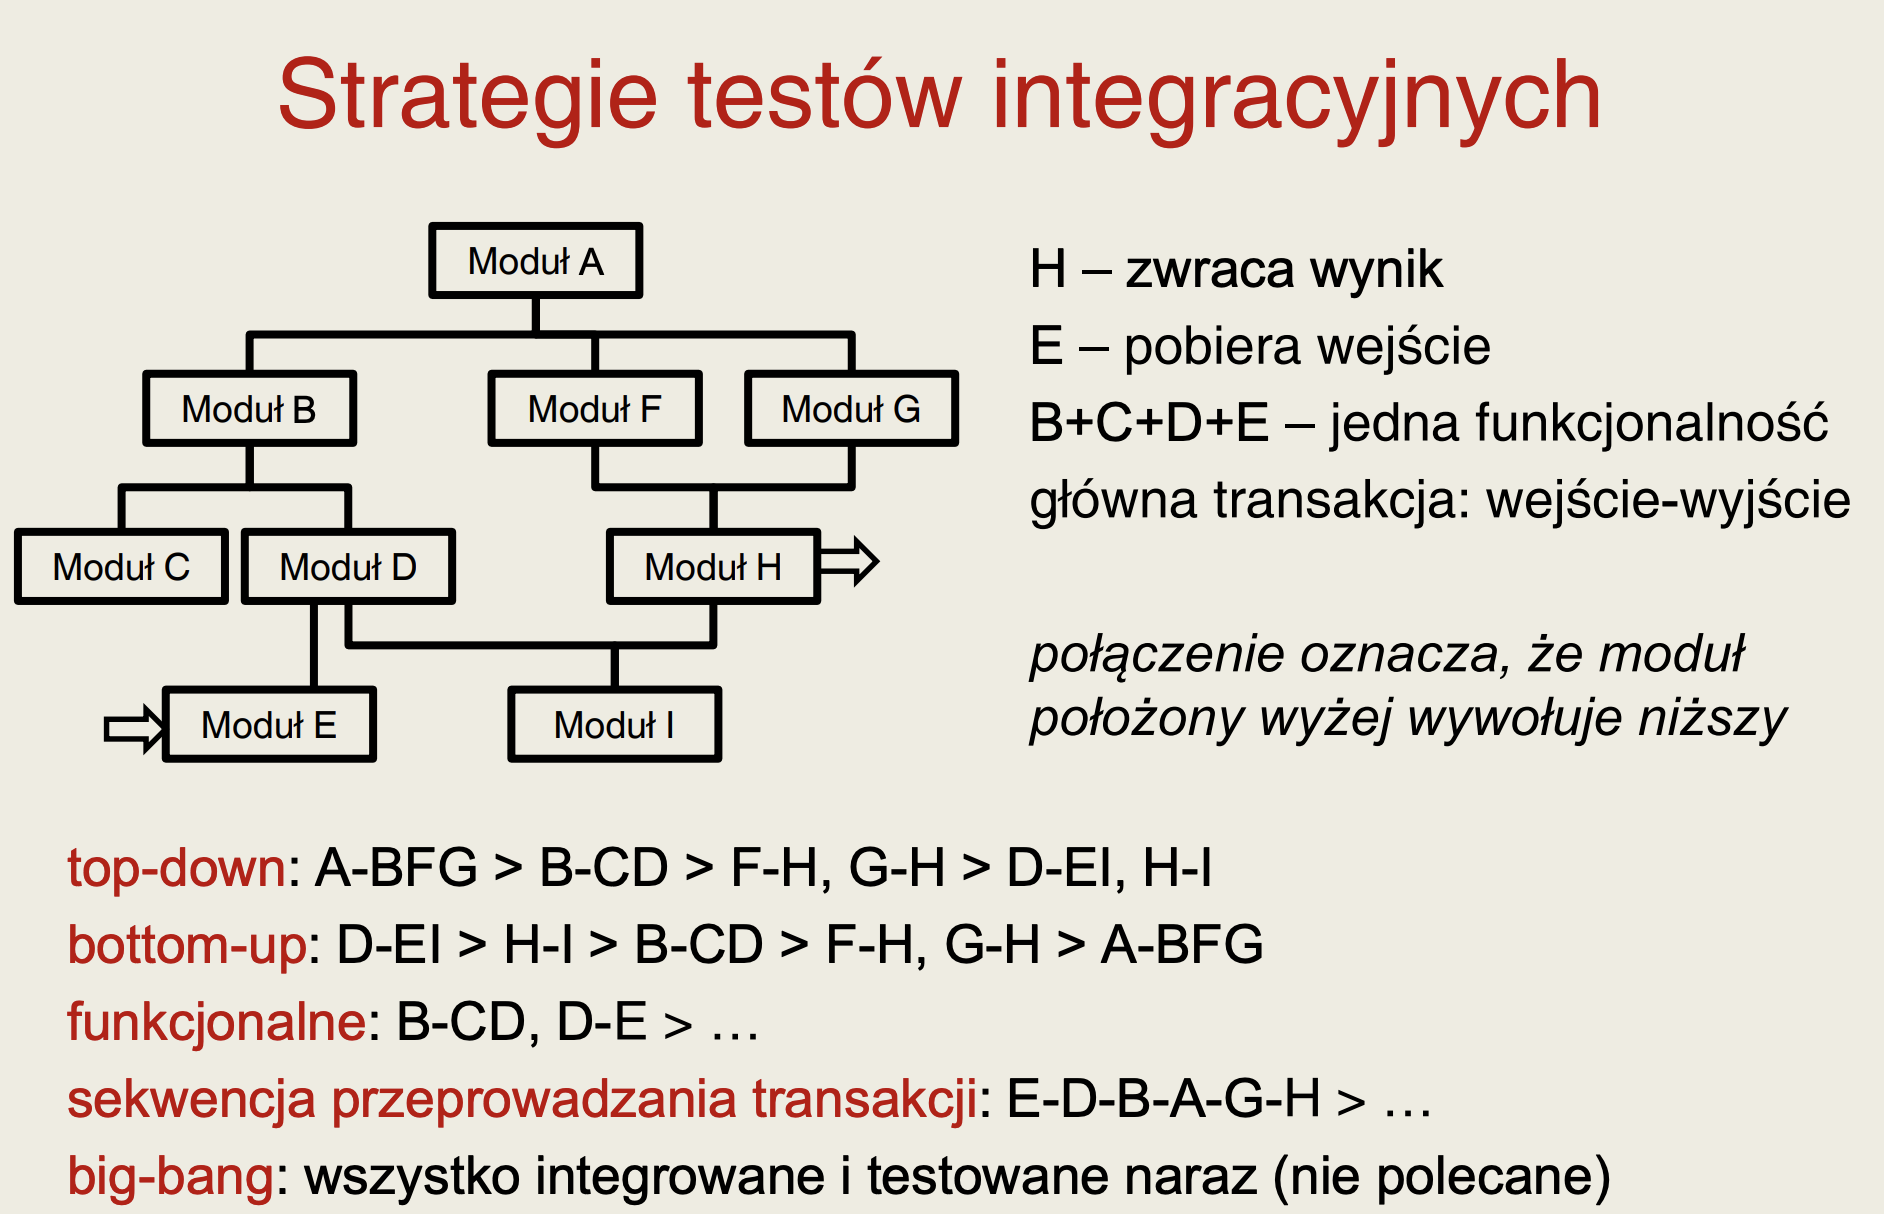
\includegraphics[width=\linewidth]{strat_integr.png}
    \end{figure}

    \subsubsection{Testy systemowe.}
    \begin{tabular}{|p{3cm}|p{13cm}|}
        \hline
        \textbf{Podstawa testów} & wymagania na system, przypadki użycia,
        specyfikacja funkcjonalna, raporty analizy ryzyka\\
        \hline
        \textbf{Typowe obiekty} & system, podręczniki użytkownika i operatora,
        konfiguracja systemu\\
        \hline
    \end{tabular}

    \begin{itemize}
        \item sprawdza zachowanie systemu jako całości
        \item zakres testu określony w planie testów
        \item środowisko testowe podobne do produkcyjnego – minimalizacja ryzyka awarii zależnych od środowiska
        \item często konieczność testowania z niekompletnymi wymaganiami
        \item zwykle przeprowadzane przez niezależny zespół testerski
    \end{itemize}


    \subsubsection{Testy akceptacyjne.}
    \begin{tabular}{|p{3cm}|p{13cm}|}
        \hline
        \textbf{Podstawa testów} & wymagania użytkownika, wymagania na system,
        przypadki użycia, procesy biznesowe, raporty
        analizy ryzyka\\
        \hline
        \textbf{Typowe obiekty} & Procesy biznesowe w pełni zintegrowanego
        systemu, procesy operacyjne i utrzymania systemu,
        procedury, raporty, dane konfiguracyjne\\
        \hline
    \end{tabular}

    \begin{itemize}
        \item cel: zyskanie zaufania do systemu
        \item znajdowanie defektów nie jest głównym celem
        \item często przeprowadzane przez klienta lub użytkownika
        \item ocenia gotowość systemu, ale niekoniecznie ostatni etap testów
    \end{itemize}

    \textbf{Typowe formy testów akceptacyjnych:}
    \begin{itemize}
        \item \textbf{testy akceptacyjne użytkownika (UAT)} – sprawdzenie gotowości do użycia
        \item \textbf{testy operacyjne (OAT)} – akceptacja przez administratora systemu (testy
        backupu, przywracania systemu, zarządzania użytkownikami, utrzymania,
        migracji danych, bezpieczeństwa itp.)
        \item \textbf{testy akceptacyjne wymagane kontraktem/regulacjami}
        \item \textbf{testy alfa, beta (polowe)}
        \begin{itemize}
            \item alfa: przeprowadzane u producenta, ale nie przez zespół deweloperski
            \item beta: przeprowadzane u klienta przez klienta/potencjalnego użytkownika
        \end{itemize}
    \end{itemize}

    \subsection{Typy testów.}

    Typ testów to zbiór czynności testowych właściwych dla weryfikacji systemu
    w oparciu o konkretny powód lub cel testów (\textbf{jak testujemy?}).

    \begin{itemize}
        \item \textbf{Testowanie funkcjonalne} - funkcja wykonywana przez oprogramowanie - \textbf{co system robi}.
        \item \textbf{Testowanie niefunkcjonalne} - niefunkcjonalna charakterystyka jakościowa, np. niezawodność
        czy użyteczność - \textbf{jak system działa}.
        \begin{itemize}
            \item przykłady: testy wydajności, obciążenia, użyteczności, utrzymania,
            niezawodności, przenaszalności, bezpieczeństwa
            \item mierzą charakterystyki jakościowe systemu
            \item wyrażalne ilościowo (np. czas odpowiedzi w testach wydajności)
            \item mogą odnosić się do modelu jakości, na przykład:
            \begin{itemize}
                \item normy: ISO 9126 – Software Product Quality, ISO 25000
                \item model zabezpieczeń (np. wg OWASP)
                \item model użyteczności (np. heurystyki Nielsena)
                \item profil operacyjny (dla testów wydajności)
            \end{itemize}
        \end{itemize}
        \item \textbf{Testowanie strukturalne} - struktura lub architektura systemu
        \begin{itemize}
            \item oparte na strukturze
            \begin{itemize}
                \item np. kod, graf przepływu sterowania, struktura menu, model procesu biznesowego
            \end{itemize}
            \item zwykle wykonywane po testach czarnoskrzynkowych, aby sprawdzić stopień przetestowania i wyrazić go
            ilościowo (pokrycie)
            \item pokrycie = stopień w jakim dana struktura została przetestowana
            \begin{itemize}
                \item wyrażane w \% pokrytych elementów
            \end{itemize}
            \item uzyskanie 100\% może być nieosiągalne
        \end{itemize}
        \item \textbf{Retesty i testy regresji} - związany ze zmianą, tzn. potwierdzenie usunięcia defektów
        (retesty) oraz poszukiwanie niezamierzonych zmian (regresja) - \textbf{związane ze zmianami}
        \begin{itemize}
            \item \textbf{regresja} = zjawisko pogarszania się jakości systemu na skutek
            wprowadzanych w nim zmian
            \item testy regresji to testy niezmienionych fragmentów programu
            po dokonaniu zmiany w programie; są naturalnym kandydatem do automatyzacji
            \item \textbf{retest} = przetestowanie naprawionego fragmentu systemu
        \end{itemize}
    \end{itemize}

    \subsection{Statyczne techniki testowania}
    Ręczne sprawdzanie (przeglądy) i automatyczna analiza (analiza statyczna) kodu lub dokumentacji
    bez uruchamiania kodu, ale zwykle z użyciem narzędzi!

    \begin{figure}[H]
        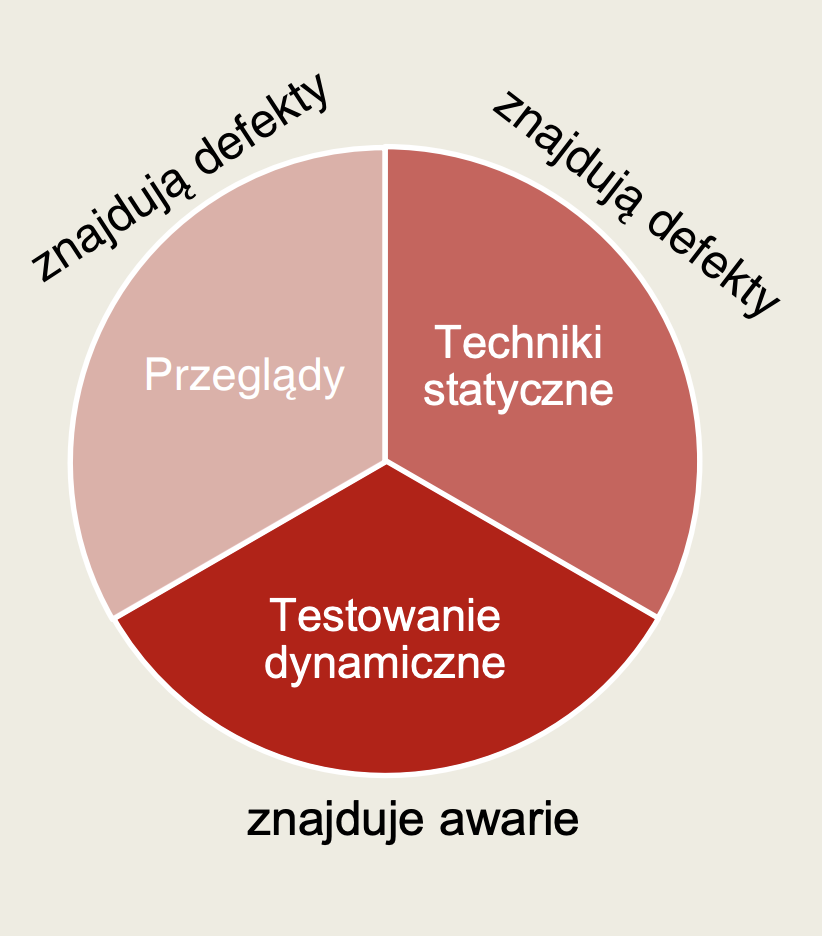
\includegraphics[width=0.5\linewidth]{metody.png}
    \end{figure}

    \subsubsection{Przeglądy.}
    \begin{itemize}
        \item Sposoby ręcznego testowania oprogramowania (np. kodu, dokumentacji)
        \item Mogą być wykonane przed fazą testów dynamicznych
        \item Pozwalają wykryć defekty wcześnie w cyklu życia (np. w wymaganiach),
        przez co usunięcie tych defektów jest tanie
        \item Aktywność manualna, ale może być wsparta narzędziami
        \item Idea: sprawdzić produkt i skomentować go
        \item Przeglądom może podlegać wszystko (specyfikacja wymagań, projekt,
        kod, plan testów, specyfikacja testów, przypadki testowe, skrypty testowe,
        podręczniki użytkownika, strony www itd.)
    \end{itemize}

    \textbf{Korzyści z przeglądów:}
    \begin{itemize}
        \item wczesne wykrycie i naprawa defektów
        \item doskonalenie jakości tworzonego kodu
        \item redukcja kosztu i czasu testów
        \item mniej defektów (w późniejszych fazach)
        \item ulepszenie komunikacji
    \end{itemize}

    \textbf{Rodzaje przeglądów}

    \begin{tabular}{|c|c|c|}
        \hline
        \textbf{Typ przeglądu} & \textbf{Charakterystyka} & \textbf{Cel}\\
        \hline
        \textbf{nieformalny} & brak formalnego procesu, może przybrać formę programowania w parach lub nieformalnej rozmowy &
        tani sposób na osiągnięcie niewielkich korzyści\\
        \hline
        \textbf{przejrzenie} & prowadzone przez autora; opcjonalne przygotowanie przed spotkaniem,
        opcjonalny raport z przeglądu & uczenie się, zrozumienie, znajdowanie usterek\\
        \hline
        \textbf{techniczny} & przeszkolony moderator, przygotowanie przed spotkaniem, zdefiniowany proces
        postępowania & podjęcie decyzji, ocena alternatyw, szukanie usterek, rozw. probl. technicznych\\
        \hline
        \textbf{inspekcja} & przeszkolony moderator, wyróżnione role i metryki, formalny proces, przygotowanie przed
        spotkaniem, formalny proces kontroli napraw & wyszukiwanie usterek\\
        \hline
    \end{tabular}

    \subsubsection{Inspekcja}

    \textbf{Role:}
    \begin{itemize}
        \item kierownik
        \item moderator
        \item autor
        \item przeglądający
        \item protokolant
    \end{itemize}

    \textbf{Proces:}
    \begin{itemize}
        \item Planowanie
        \item Rozpoczęcie
        \item Przygotowanie indywidualne
        \item Kontrola/ocena/zapis wyników
        \item Poprawki
        \item Zakończenie
    \end{itemize}

    \subsection{Projektowanie testów.}
    \begin{figure}[H]
        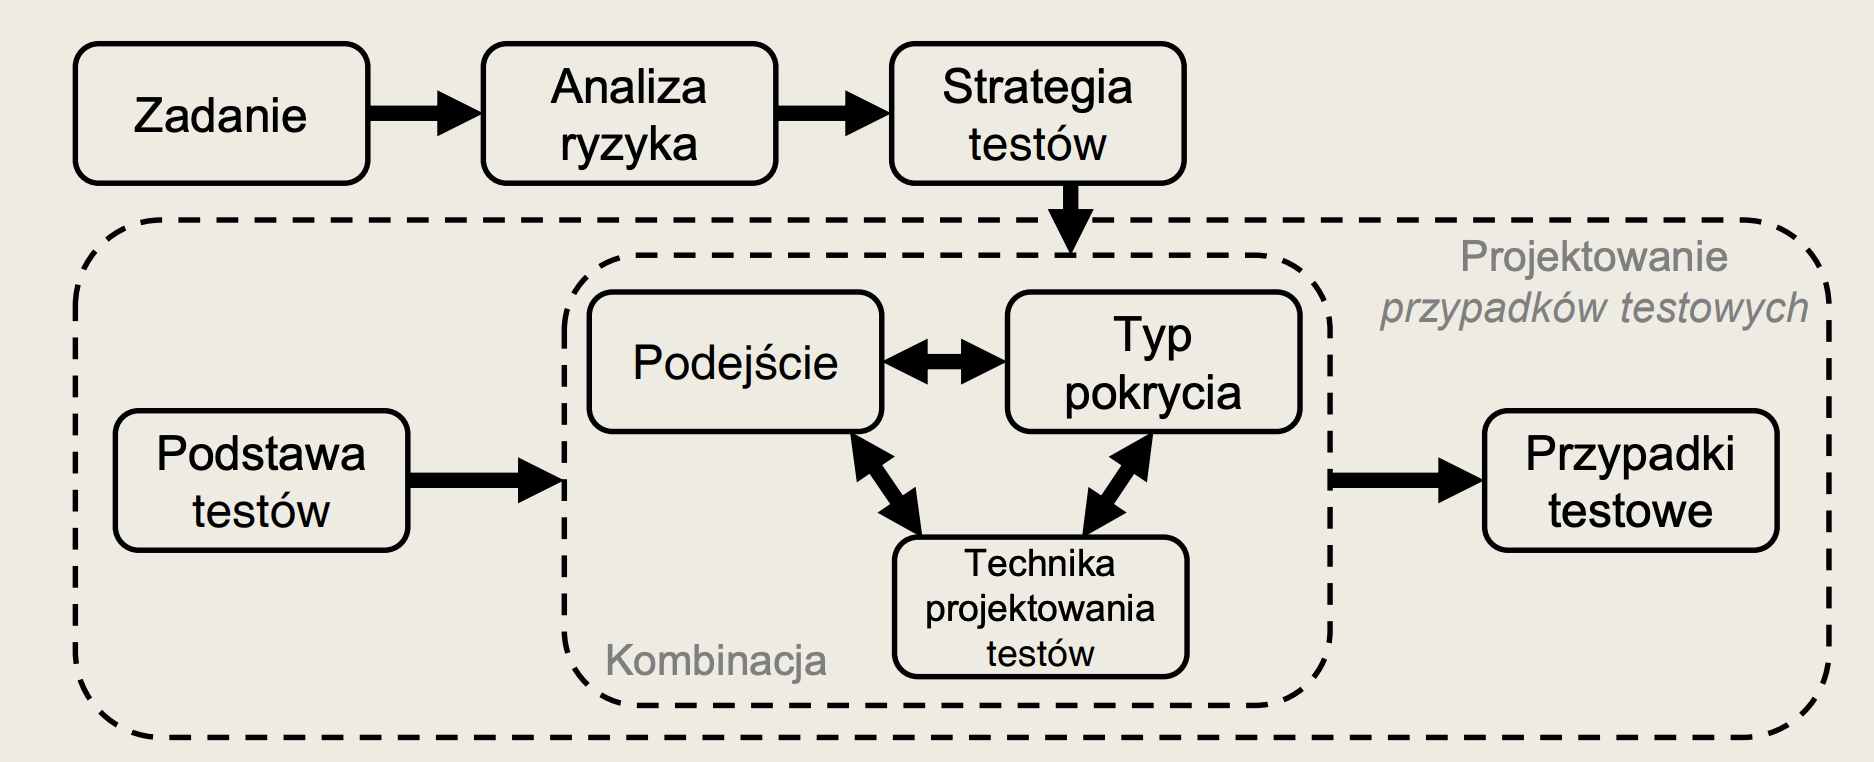
\includegraphics[width=\linewidth]{projektowanie.png}
    \end{figure}
    \begin{figure}[H]
        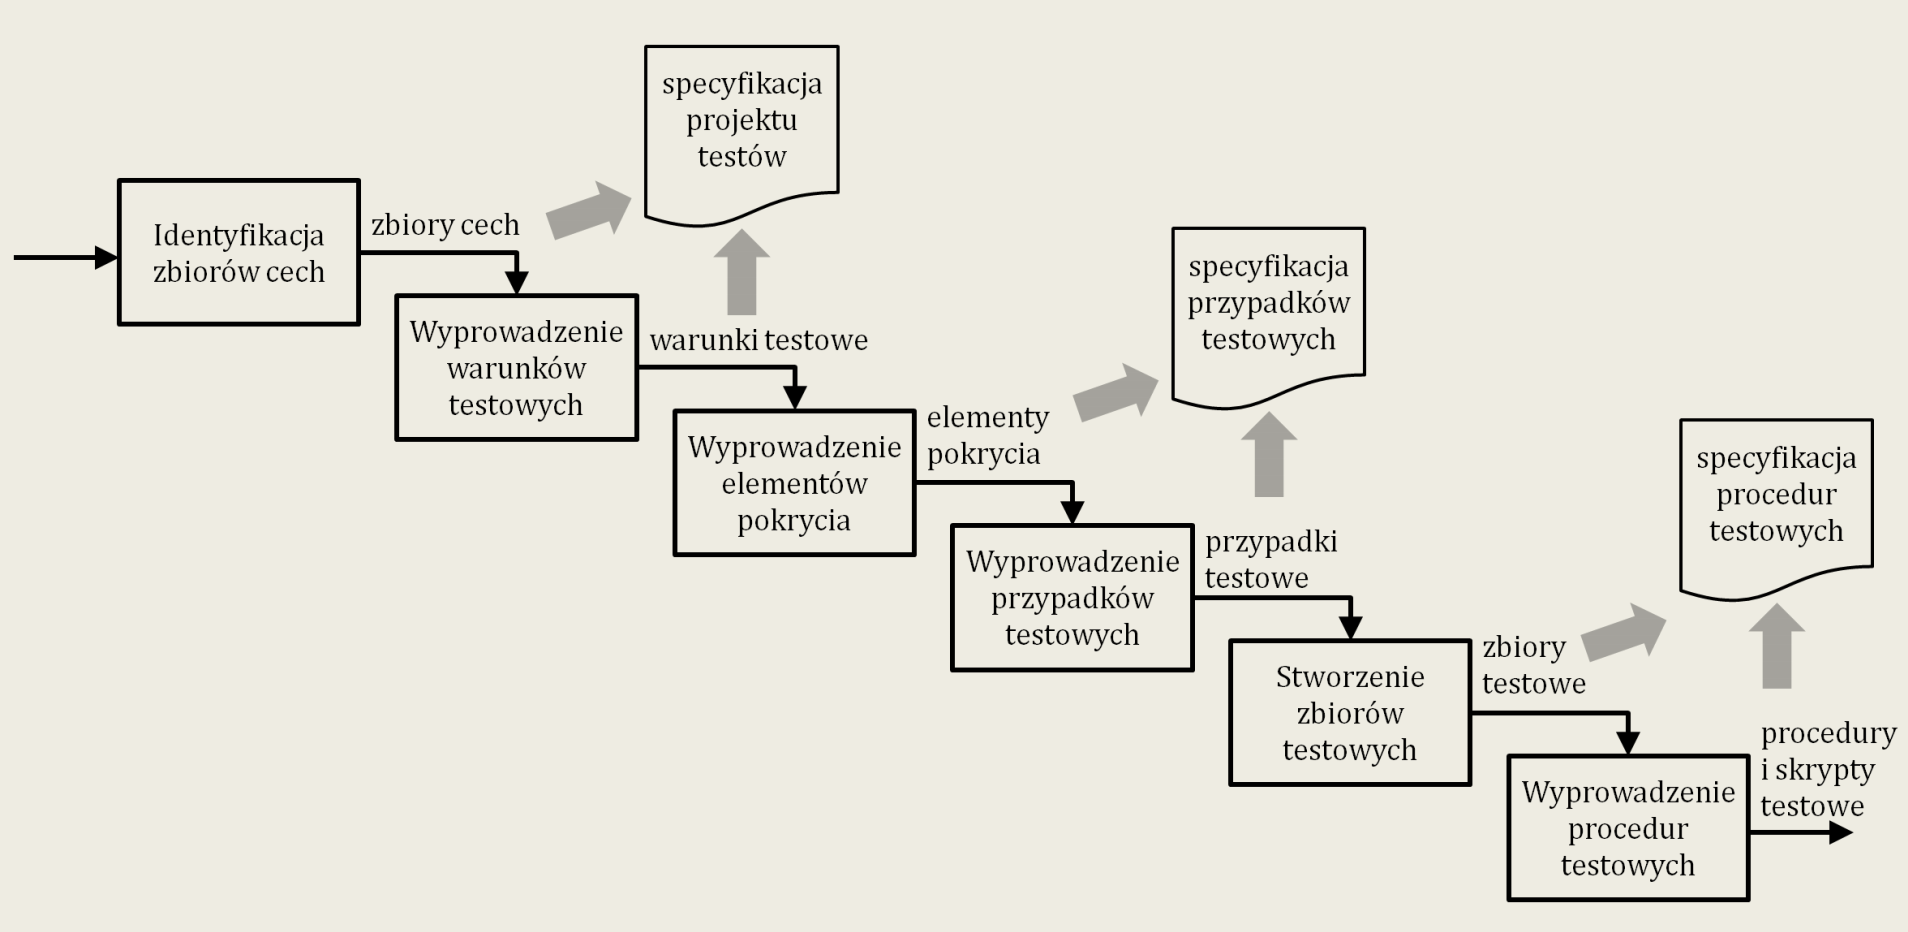
\includegraphics[width=\linewidth]{projektowanie29119.png}
    \end{figure}


    \textbf{Warunek testowy} (test condition) – element lub zdarzenie które może być
    sprawdzone przez jeden lub więcej przypadków testowych (np. funkcja,
    transakcja, atrybut jakościowy, element strukturalny).

    \textbf{Element pokrycia} (coverage item) – element lub zdarzenie używane jako
    podstawa dla pokrycia testu (np. przejście w maszynie stanów, instrukcja
    kodu).

    \textbf{Przypadek testowy} - generyczna struktura: warunki początkowe, działanie i wynik = wejście, przetwarzanie, wyjście.

    \begin{figure}[H]
        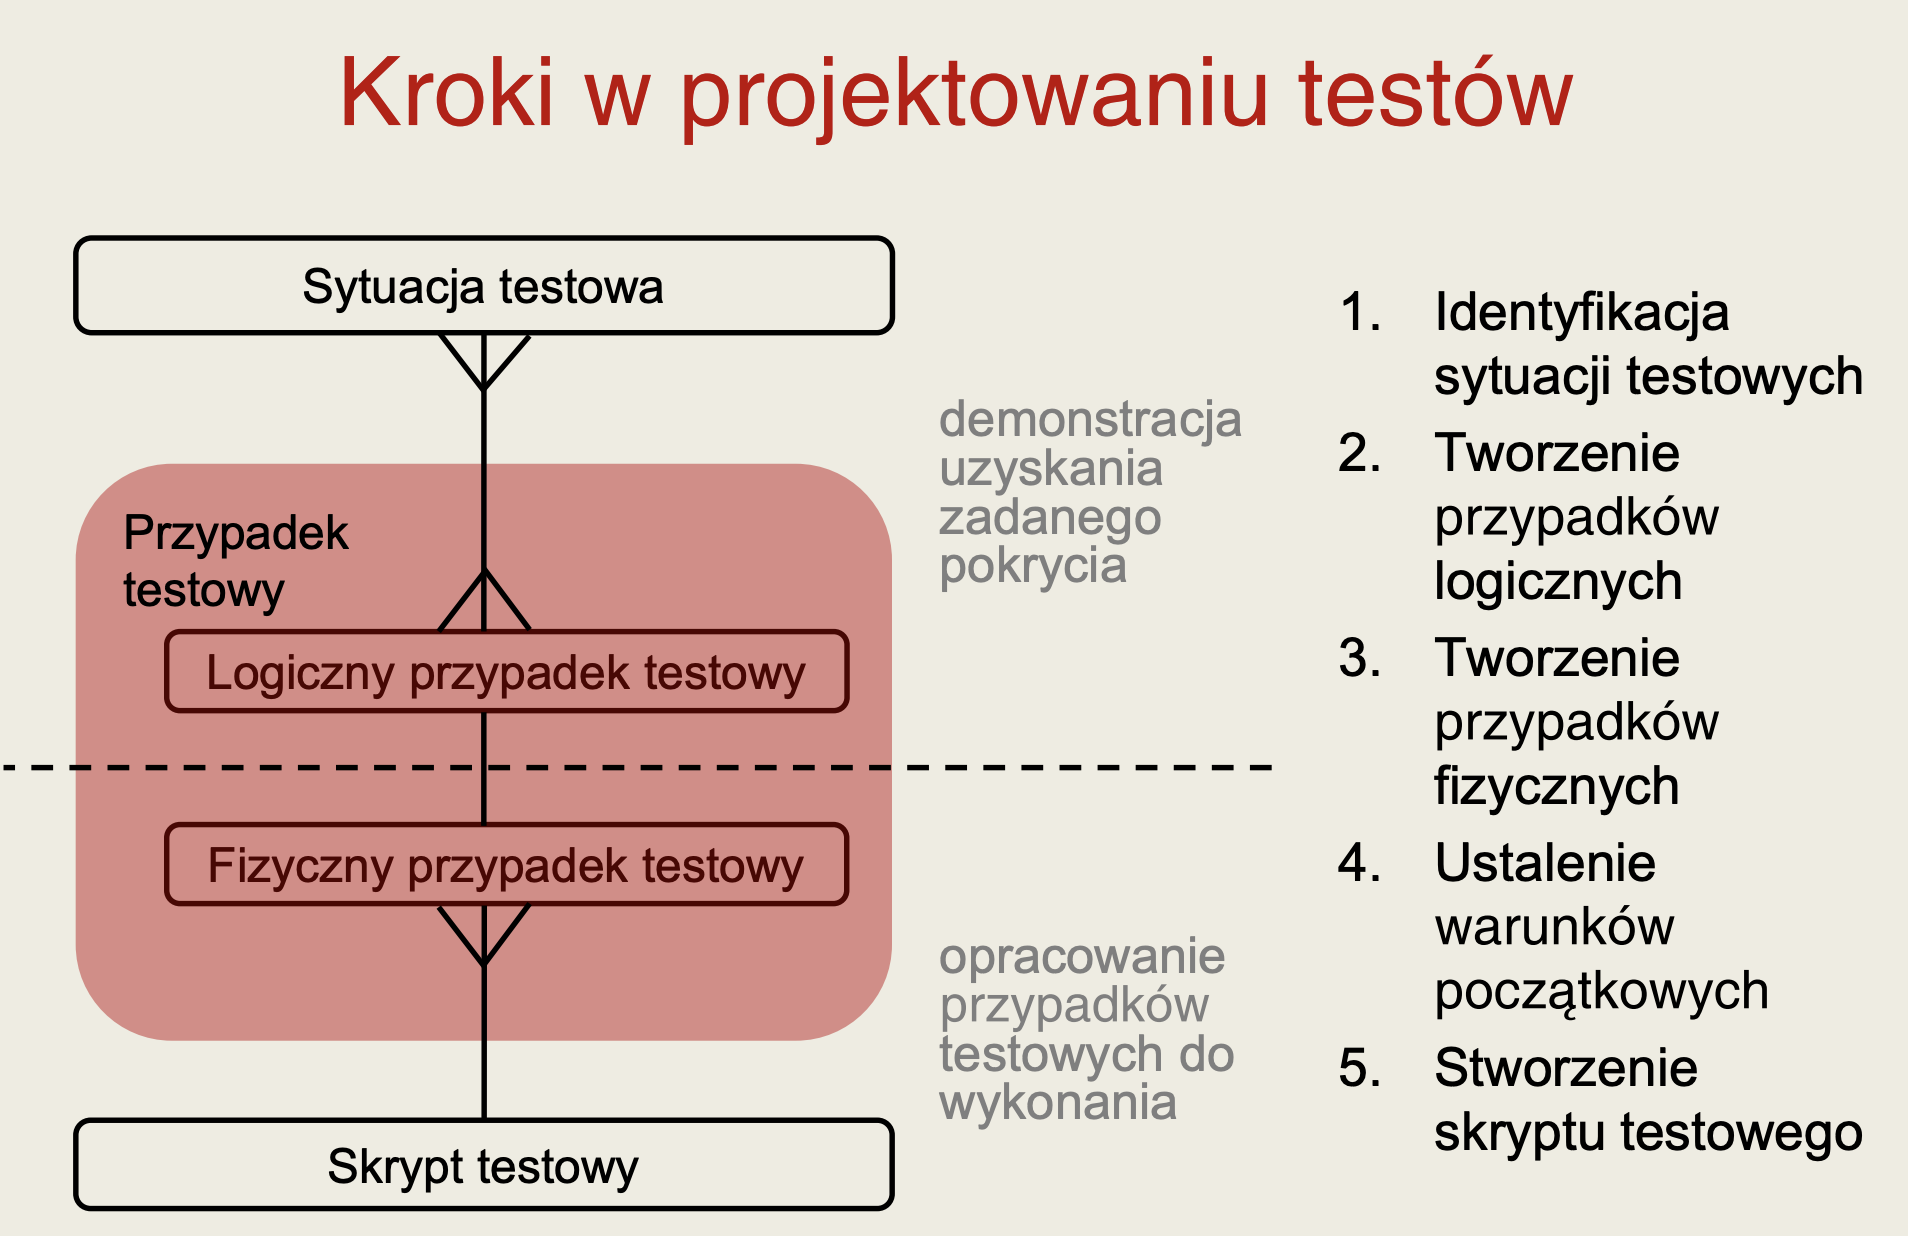
\includegraphics[width=\linewidth]{projektowaniekroki.png}
    \end{figure}
\end{document}